\chapter{Portfolio Optimization: Markowitz and Beyond}
\label{ch:portfolio}

\begin{companioncode}{quant-portfolio}
Code: \texttt{crates/quant-portfolio/}\\
Dependencies: \crate{quant-core}, \crate{quant-timeseries}, \crate{thiserror}\\
Run: \texttt{cargo run -p quant-portfolio --example frontier}
\end{companioncode}

\section{Learning Objectives}

This chapter builds the Markowitz mean-variance framework on top of the
returns and covariance machinery from \cref{ch:returns} and \cref{ch:timeseries}:
the efficient frontier, the global minimum-variance portfolio, the tangency
portfolio, the capital market line, two-fund separation, and CAPM. After
completing it you can:

\begin{itemize}
    \item State the Markowitz mean-variance optimisation problem and its
      Lagrangian dual
    \item Compute the two-asset efficient frontier in closed form and
      identify the minimum-varance weight
    \item Solve the $n$-asset minimum-variance and target-return portfolios
      via the inverse of the covariance matrix
    \item Derive the tangency portfolio (maximum Sharpe) in closed form and
      draw the capital market line
    \item Apply two-fund separation: any efficient portfolio is a mix of the
      risk-free asset and the tangency portfolio
    \item Estimate CAPM beta and Jensen's alpha from a return series and
      interpret them on the security market line
    \item Compute historical Value-at-Risk and Conditional VaR
\end{itemize}

\begin{keyinsight}
Diversification is the only free lunch in finance. The efficient frontier
is the set of portfolios that maximise expected return for a given variance
(or minimise variance for a given return). The tangency portfolio is the
point on the frontier that maximises the Sharpe ratio; once a risk-free
asset exists, every efficient portfolio is a mix of the risk-free asset
and the tangency portfolio --- the celebrated \emph{two-fund separation}
theorem.
\end{keyinsight}

\section{The Markowitz Problem}

\marginnote{%
\textbf{Markowitz in one sentence}\\[0.3em]
For each target return, pick the portfolio of minimum variance that
achieves it. Sweep the target to trace the efficient frontier. The
recipe is 70 years old and still the starting point of every
portfolio construction problem.
}

Consider $n$ risky assets with expected return vector $\mu$ and covariance
matrix $\Sigma$. A portfolio is a vector of weights $w \in \mathbb{R}^n$
with budget constraint $1^\top w = 1$. The portfolio return and variance are
\[
\mu_p = w^\top \mu, \qquad \sigma_p^2 = w^\top \Sigma w.
\]
The Markowitz problem is to find, for each target return $\mu_\star$, the
portfolio that achieves it at minimum variance:
\[
\min_w \; w^\top \Sigma w
\quad \text{s.t.} \quad
1^\top w = 1, \;\; \mu^\top w = \mu_\star.
\]
The set of solutions, swept over $\mu_\star$, is the \emph{efficient
frontier}. Without a risk-free asset the frontier is a hyperbola in
$(\sigma_p, \mu_p)$ space; with a risk-free asset the relevant efficient set
becomes the straight line from $(0, r_f)$ through the tangency portfolio.

The \func{Portfolio} struct carries the three inputs (weights, expected
returns, covariance) together and exposes the three headline statistics:

\begin{lstlisting}[language=Rust]
pub struct Portfolio {
    pub weights: Vec<f64>,
    pub expected_returns: Vec<f64>,
    pub covariance: Vec<Vec<f64>>,
}

impl Portfolio {
    pub fn expected_return(&self) -> f64 {
        self.weights.iter()
            .zip(self.expected_returns.iter())
            .map(|(w, m)| w * m).sum()
    }
    pub fn variance(&self) -> f64 {
        quadratic_form(&self.weights, &self.covariance)
    }
    pub fn volatility(&self) -> f64 { self.variance().sqrt() }
    pub fn sharpe(&self, rf: f64) -> f64 {
        let vol = self.volatility();
        if vol == 0.0 { 0.0 } else { (self.expected_return() - rf) / vol }
    }
}
\end{lstlisting}

The quadratic form $w^\top \Sigma w$ is a one-liner once a matrix-vector
product is available; the Sharpe ratio guards against a zero-volatility
degenerate portfolio (all cash).

\section{Two-Asset Closed-Form Frontier}

\marginnote{%
\textbf{Two-asset frontier}\\[0.3em]
$\mu_p = w \mu_A + (1{-}w) \mu_B$\\[0.2em]
$\sigma_p^2 = w^2 \sigma_A^2 + (1{-}w)^2 \sigma_B^2 + 2 w (1{-}w) \rho \sigma_A \sigma_B$\\[0.3em]
\textbf{Min-variance weight}\\[0.2em]
$w_A^\star = \dfrac{\sigma_B^2 - \rho \sigma_A \sigma_B}{\sigma_A^2 + \sigma_B^2 - 2 \rho \sigma_A \sigma_B}$
}

For two assets the frontier is a single-parameter curve indexed by the
weight $w$ on asset A. The minimum-variance weight has a closed form that
falls out of setting $d\sigma_p^2 / dw = 0$:
\[
w_A^\star = \frac{\sigma_B^2 - \rho \sigma_A \sigma_B}
                 {\sigma_A^2 + \sigma_B^2 - 2 \rho \sigma_A \sigma_B}.
\]
Three boundary cases are worth knowing by heart:
\begin{itemize}
    \item $\rho = 0$: $w_A^\star = \sigma_B^2 / (\sigma_A^2 + \sigma_B^2)$
      --- the inverse-variance weights.
    \item $\rho = 1$ and $\sigma_A = \sigma_B$: any split has the same
      variance; the formula is degenerate ($0/0$), so we fall back to
      $w_A^\star = 1/2$.
    \item $\rho = -1$: a perfect hedge exists; the minimum variance is
      zero (a risk-free portfolio can be synthesised from two risky
      assets).
\end{itemize}

\begin{lstlisting}[language=Rust]
pub fn two_asset_min_variance_weight(
    var_a: f64, var_b: f64, cov_ab: f64,
) -> f64 {
    let denom = var_a + var_b - 2.0 * cov_ab;
    if denom.abs() < 1e-15 { return 0.5; }  // degenerate
    (var_b - cov_ab) / denom
}

pub fn two_asset_frontier_point(
    w: f64, mu_a: f64, mu_b: f64,
    var_a: f64, var_b: f64, cov_ab: f64,
) -> FrontierPoint {
    let mu_p = w * mu_a + (1.0 - w) * mu_b;
    let var_p = w * w * var_a
        + (1.0 - w) * (1.0 - w) * var_b
        + 2.0 * w * (1.0 - w) * cov_ab;
    FrontierPoint { expected_return: mu_p, volatility: var_p.sqrt() }
}
\end{lstlisting}

The degenerate case (equal variances, $\rho = 1$) returns $w = 1/2$ rather
than panicking on a $0/0$ --- any split is minimum-variance when the assets
are perfectly correlated and equally volatile.

\section{The $n$-Asset Lagrangian}

\marginnote{%
\textbf{Why closed form?}\\[0.3em]
With only equality constraints ($1^\top w = 1$, $\mu^\top w =
\mu_\star$) the KKT system is linear: $2\Sigma w = \lambda_1 1 +
\lambda_2 \mu$. Inverting $\Sigma$ once gives every frontier
portfolio as a linear combination of $\Sigma^{-1} 1$ and
$\Sigma^{-1} \mu$. Inequality constraints (no short sales, box
constraints) destroy this closed form and require a real QP solver.
}

For $n$ assets the Markowitz problem is a constrained quadratic program.
With no inequality constraints (short sales allowed), the KKT conditions
reduce to a linear system and everything has a closed form in terms of
$\Sigma^{-1}$.

\subsection{Global Minimum-Variance Portfolio}

Minimising $w^\top \Sigma w$ subject only to $1^\top w = 1$ has the
Lagrangian $\mathcal{L} = w^\top \Sigma w - \lambda (1^\top w - 1)$, whose
stationarity gives $\Sigma w = \lambda 1$ and the budget constraint
recovers $\lambda$. The closed form is
\[
w^\star_{\text{GMV}} = \frac{\Sigma^{-1} 1}{1^\top \Sigma^{-1} 1}.
\]

\subsection{Efficient Frontier at a Target Return}

Adding the return constraint $\mu^\top w = \mu_\star$ produces a second
Lagrange multiplier. Define the standard scalars
\[
a = 1^\top \Sigma^{-1} 1, \quad
b = 1^\top \Sigma^{-1} \mu, \quad
c = \mu^\top \Sigma^{-1} \mu, \quad
d = a c - b^2.
\]
Then the target-return efficient portfolio is
\[
w^\star(\mu_\star) = \frac{1}{d} \, \Sigma^{-1}
\bigl[ (c - b \mu_\star) 1 + (a \mu_\star - b) \mu \bigr],
\]
and the minimum variance achievable for that target is
\[
\sigma_p^2(\mu_\star) = \frac{a \mu_\star^2 - 2 b \mu_\star + c}{d}.
\]
This is a parabola in $(\mu_\star, \sigma_p^2)$ space, opening upward; its
tip is the global minimum-variance portfolio at $\mu_\star = b/a$ with
variance $1/a$.

\begin{lstlisting}[language=Rust]
pub fn min_variance_portfolio(
    expected_returns: &[f64],
    covariance: &[Vec<f64>],
) -> Result<Vec<f64>, PortfolioError> {
    let n = expected_returns.len();
    let sigma_inv = inverse(covariance)?;
    let ones = vec![1.0_f64; n];
    let sigma_inv_ones = matvec(&sigma_inv, &ones);
    let denom: f64 = sigma_inv_ones.iter().sum();
    Ok(sigma_inv_ones.iter().map(|v| v / denom).collect())
}

pub fn efficient_frontier_point(
    expected_returns: &[f64],
    covariance: &[Vec<f64>],
    mu_target: f64,
) -> Result<Vec<f64>, PortfolioError> {
    let sigma_inv = inverse(covariance)?;
    let ones = vec![1.0_f64; expected_returns.len()];
    let sigma_inv_ones = matvec(&sigma_inv, &ones);
    let sigma_inv_mu = matvec(&sigma_inv, expected_returns);
    let a: f64 = sigma_inv_ones.iter().sum();
    let b: f64 = sigma_inv_ones.iter()
        .zip(expected_returns.iter()).map(|(x, m)| x * m).sum();
    let c: f64 = expected_returns.iter()
        .zip(sigma_inv_mu.iter()).map(|(m, x)| m * x).sum();
    let d = a * c - b * b;
    let coef_ones = (c - b * mu_target) / d;
    let coef_mu = (a * mu_target - b) / d;
    Ok((0..expected_returns.len())
        .map(|i| coef_ones * sigma_inv_ones[i] + coef_mu * sigma_inv_mu[i])
        .collect())
}
\end{lstlisting}

Both functions hinge on the small Gaussian-elimination \func{inverse}
in \crate{quant-portfolio}'s \func{linalg} module --- the only linear
algebra primitive needed for the entire Markowitz framework. The budget
constraint is implicit in the closed form: the numerator of
\func{min\_variance\_portfolio} is $\Sigma^{-1} 1$ (unnormalised), and
dividing by $1^\top \Sigma^{-1} 1$ enforces $\sum w_i = 1$.

\section{The Tangency Portfolio}

\marginnote{%
\textbf{Tangency portfolio}\\[0.3em]
$w^\star_{\text{tan}} = \dfrac{\Sigma^{-1} (\mu - r_f 1)}{1^\top \Sigma^{-1} (\mu - r_f 1)}$\\[0.3em]
\textbf{Sharpe}\\[0.2em]
$\text{Sharpe} = \dfrac{\mu_p - r_f}{\sigma_p}$
}

With a risk-free rate $r_f$, every efficient portfolio is a mix of the
risk-free asset and a single risky portfolio: the \emph{tangency
portfolio}, the point on the efficient frontier that maximises the Sharpe
ratio. The closed form is
\[
w^\star_{\text{tan}} = \frac{\Sigma^{-1} (\mu - r_f 1)}{1^\top \Sigma^{-1} (\mu - r_f 1)}.
\]
The numerator is the direction that maximises the excess-return-to-variance
trade-off; the denominator normalises the budget to one. If all expected
returns equal $r_f$ the tangency is undefined (the excess return vector is
zero) and we surface an error.

\begin{lstlisting}[language=Rust]
let excess: Vec<f64> = expected_returns.iter().map(|m| m - rf).collect();
let sigma_inv = inverse(covariance)?;
let sigma_inv_excess = matvec(&sigma_inv, &excess);
let denom: f64 = sigma_inv_excess.iter().sum();
let weights: Vec<f64> = sigma_inv_excess.iter().map(|v| v / denom).collect();
\end{lstlisting}

\section{The Capital Market Line and Two-Fund Separation}

\marginnote{%
\textbf{Capital market line}\\[0.3em]
$\mu_p = r_f + \text{Sharpe}_{\text{tan}} \cdot \sigma_p$\\[0.3em]
\textbf{Two-fund separation}\\[0.2em]
$y = \sigma_p / \sigma_{\text{tan}}$\\
$w = y \, w_{\text{tan}} + (1{-}y) \, r_f$
}

The capital market line (CML) is the straight line in $(\sigma, \mu)$
space from $(0, r_f)$ through the tangency point:
\[
\mu_p = r_f + \text{Sharpe}_{\text{tan}} \cdot \sigma_p.
\]
Every point on the CML is achievable by mixing the risk-free asset with
the tangency portfolio. The fraction invested in the tangency portfolio
to achieve a target volatility $\sigma_p$ is $y = \sigma_p / \sigma_{\tan}$;
the rest, $1 - y$, is invested at $r_f$. This is the
\emph{two-fund separation} theorem: investors with different risk
preferences differ only in $y$, not in the composition of the risky
fund. The tangency portfolio is the market portfolio under CAPM
assumptions.

\begin{marginfigure}
    \centering
    \vspace{-3cm}
    % Markowitz Efficient Frontier with Tangency Portfolio and CML
% Usage: % Markowitz Efficient Frontier with Tangency Portfolio and CML
% Usage: % Markowitz Efficient Frontier with Tangency Portfolio and CML
% Usage: \input{figures/efficient-frontier}
% Coordinates: scale_x = 20 (sigma in [0, 0.30] -> 0..6 cm)
%              scale_y = 50 (mu    in [0, 0.12] -> 0..6 cm)
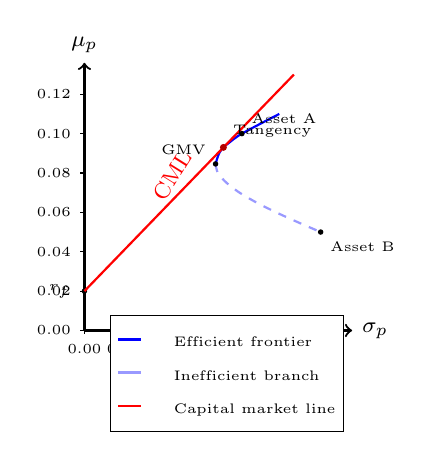
\begin{tikzpicture}[scale=0.5]
    % Axes (clipped to chart area: x in [0, 6.5], y in [0, 6.5])
    \draw[thick, ->] (0,0) -- (6.8,0) node[right] {\footnotesize $\sigma_p$};
    \draw[thick, ->] (0,0) -- (0,6.8) node[above] {\footnotesize $\mu_p$};

    % Chart border (light, optional) to visualise the plot area
    % \draw[gray!30, very thin] (0,0) rectangle (6.5,6.5);

    % Tick labels on x-axis (volatility)
    \foreach \x/\xlab in {0/0.00, 1/0.05, 2/0.10, 3/0.15, 4/0.20, 5/0.25, 6/0.30} {
        \draw (\x,0) -- (\x,-0.1);
        \node[below] at (\x,-0.1) {\tiny \xlab};
    }
    % Tick labels on y-axis (expected return)
    \foreach \y/\ylab in {0/0.00, 1/0.02, 2/0.04, 3/0.06, 4/0.08, 5/0.10, 6/0.12} {
        \draw (0,\y) -- (-0.1,\y);
        \node[left] at (-0.1,\y) {\tiny \ylab};
    }

    % Risk-free rate point on the y-axis
    \fill[black] (0,1.0) circle (2pt);
    \node[left] at (-0.1,1.0) {\tiny $r_f$};

    % Efficient frontier (upper branch of the risky-assets hyperbola).
    % Starts at GMV (w = w_GMV) and rises through the tangency portfolio
    % to asset A and beyond (short B to leverage A).
    \draw[thick, blue] plot[smooth] coordinates {
        (3.33,4.23) (3.42,4.50) (3.53,4.65) (3.65,4.75)
        (4.00,5.00) (4.95,5.50)
    };

    % Inefficient lower branch (w < w_GMV): same variance as the upper
    % branch, but lower return. Runs from GMV down-right to asset B
    % (all-B portfolio) and beyond (short A to buy more B).
    \draw[thick, blue!40, dashed] plot[smooth] coordinates {
        (3.33,4.23) (3.39,4.00) (3.61,3.75) (3.94,3.50)
        (4.37,3.25) (4.87,3.00) (5.42,2.75) (6.00,2.50)
    };

    % Capital market line: from (0, rf) through tangency, clipped at y=6.5.
    % Slope in scaled coords: (4.65-1.0)/(3.53-0) = 1.034.
    % At y=6.5: x = (6.5-1.0)/1.034 = 5.318.
    \draw[thick, red] (0,1.0) -- (5.32, 6.5);
    \node[red, above, rotate=58] at (2.6, 3.7) {\footnotesize CML};

    % Asset points
    \fill[black] (4.00,5.00) circle (2pt);
    \node[above right] at (4.00,5.00) {\tiny Asset A};
    \fill[black] (6.00,2.50) circle (2pt);
    \node[below right] at (6.00,2.50) {\tiny Asset B};

    % Global minimum-variance portfolio
    \fill[black] (3.33,4.23) circle (2pt);
    \node[above left] at (3.33,4.23) {\tiny GMV};

    % Tangency portfolio
    \fill[red!70!black] (3.53,4.65) circle (2.5pt);
    \node[above right] at (3.53,4.65) {\tiny Tangency};

    % Legend in the lower-right empty area (below the inefficient branch).
    \node[draw, fill=white, inner sep=3pt, anchor=north east]
        at (6.6, 0.4) {%
        \begin{tabular}{@{}ll@{}}
            \textcolor{blue}{\rule[0.5ex]{8pt}{1pt}} & \tiny Efficient frontier \\
            \textcolor{blue!40}{\rule[0.5ex]{8pt}{1pt}} & \tiny Inefficient branch \\
            \textcolor{red}{\rule[0.5ex]{8pt}{1pt}} & \tiny Capital market line \\
        \end{tabular}};
\end{tikzpicture}
% Coordinates: scale_x = 20 (sigma in [0, 0.30] -> 0..6 cm)
%              scale_y = 50 (mu    in [0, 0.12] -> 0..6 cm)
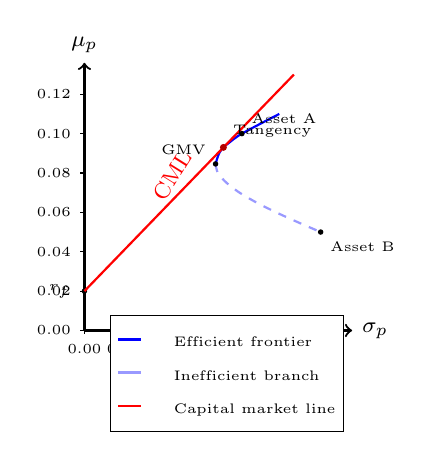
\begin{tikzpicture}[scale=0.5]
    % Axes (clipped to chart area: x in [0, 6.5], y in [0, 6.5])
    \draw[thick, ->] (0,0) -- (6.8,0) node[right] {\footnotesize $\sigma_p$};
    \draw[thick, ->] (0,0) -- (0,6.8) node[above] {\footnotesize $\mu_p$};

    % Chart border (light, optional) to visualise the plot area
    % \draw[gray!30, very thin] (0,0) rectangle (6.5,6.5);

    % Tick labels on x-axis (volatility)
    \foreach \x/\xlab in {0/0.00, 1/0.05, 2/0.10, 3/0.15, 4/0.20, 5/0.25, 6/0.30} {
        \draw (\x,0) -- (\x,-0.1);
        \node[below] at (\x,-0.1) {\tiny \xlab};
    }
    % Tick labels on y-axis (expected return)
    \foreach \y/\ylab in {0/0.00, 1/0.02, 2/0.04, 3/0.06, 4/0.08, 5/0.10, 6/0.12} {
        \draw (0,\y) -- (-0.1,\y);
        \node[left] at (-0.1,\y) {\tiny \ylab};
    }

    % Risk-free rate point on the y-axis
    \fill[black] (0,1.0) circle (2pt);
    \node[left] at (-0.1,1.0) {\tiny $r_f$};

    % Efficient frontier (upper branch of the risky-assets hyperbola).
    % Starts at GMV (w = w_GMV) and rises through the tangency portfolio
    % to asset A and beyond (short B to leverage A).
    \draw[thick, blue] plot[smooth] coordinates {
        (3.33,4.23) (3.42,4.50) (3.53,4.65) (3.65,4.75)
        (4.00,5.00) (4.95,5.50)
    };

    % Inefficient lower branch (w < w_GMV): same variance as the upper
    % branch, but lower return. Runs from GMV down-right to asset B
    % (all-B portfolio) and beyond (short A to buy more B).
    \draw[thick, blue!40, dashed] plot[smooth] coordinates {
        (3.33,4.23) (3.39,4.00) (3.61,3.75) (3.94,3.50)
        (4.37,3.25) (4.87,3.00) (5.42,2.75) (6.00,2.50)
    };

    % Capital market line: from (0, rf) through tangency, clipped at y=6.5.
    % Slope in scaled coords: (4.65-1.0)/(3.53-0) = 1.034.
    % At y=6.5: x = (6.5-1.0)/1.034 = 5.318.
    \draw[thick, red] (0,1.0) -- (5.32, 6.5);
    \node[red, above, rotate=58] at (2.6, 3.7) {\footnotesize CML};

    % Asset points
    \fill[black] (4.00,5.00) circle (2pt);
    \node[above right] at (4.00,5.00) {\tiny Asset A};
    \fill[black] (6.00,2.50) circle (2pt);
    \node[below right] at (6.00,2.50) {\tiny Asset B};

    % Global minimum-variance portfolio
    \fill[black] (3.33,4.23) circle (2pt);
    \node[above left] at (3.33,4.23) {\tiny GMV};

    % Tangency portfolio
    \fill[red!70!black] (3.53,4.65) circle (2.5pt);
    \node[above right] at (3.53,4.65) {\tiny Tangency};

    % Legend in the lower-right empty area (below the inefficient branch).
    \node[draw, fill=white, inner sep=3pt, anchor=north east]
        at (6.6, 0.4) {%
        \begin{tabular}{@{}ll@{}}
            \textcolor{blue}{\rule[0.5ex]{8pt}{1pt}} & \tiny Efficient frontier \\
            \textcolor{blue!40}{\rule[0.5ex]{8pt}{1pt}} & \tiny Inefficient branch \\
            \textcolor{red}{\rule[0.5ex]{8pt}{1pt}} & \tiny Capital market line \\
        \end{tabular}};
\end{tikzpicture}
% Coordinates: scale_x = 20 (sigma in [0, 0.30] -> 0..6 cm)
%              scale_y = 50 (mu    in [0, 0.12] -> 0..6 cm)
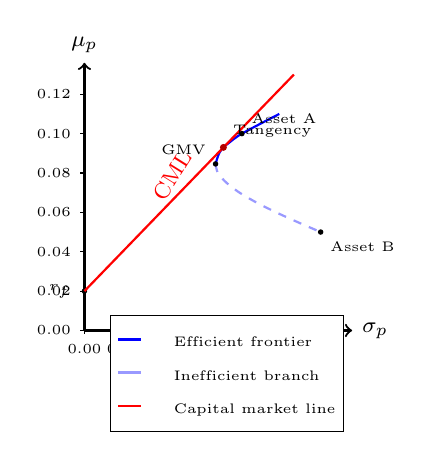
\begin{tikzpicture}[scale=0.5]
    % Axes (clipped to chart area: x in [0, 6.5], y in [0, 6.5])
    \draw[thick, ->] (0,0) -- (6.8,0) node[right] {\footnotesize $\sigma_p$};
    \draw[thick, ->] (0,0) -- (0,6.8) node[above] {\footnotesize $\mu_p$};

    % Chart border (light, optional) to visualise the plot area
    % \draw[gray!30, very thin] (0,0) rectangle (6.5,6.5);

    % Tick labels on x-axis (volatility)
    \foreach \x/\xlab in {0/0.00, 1/0.05, 2/0.10, 3/0.15, 4/0.20, 5/0.25, 6/0.30} {
        \draw (\x,0) -- (\x,-0.1);
        \node[below] at (\x,-0.1) {\tiny \xlab};
    }
    % Tick labels on y-axis (expected return)
    \foreach \y/\ylab in {0/0.00, 1/0.02, 2/0.04, 3/0.06, 4/0.08, 5/0.10, 6/0.12} {
        \draw (0,\y) -- (-0.1,\y);
        \node[left] at (-0.1,\y) {\tiny \ylab};
    }

    % Risk-free rate point on the y-axis
    \fill[black] (0,1.0) circle (2pt);
    \node[left] at (-0.1,1.0) {\tiny $r_f$};

    % Efficient frontier (upper branch of the risky-assets hyperbola).
    % Starts at GMV (w = w_GMV) and rises through the tangency portfolio
    % to asset A and beyond (short B to leverage A).
    \draw[thick, blue] plot[smooth] coordinates {
        (3.33,4.23) (3.42,4.50) (3.53,4.65) (3.65,4.75)
        (4.00,5.00) (4.95,5.50)
    };

    % Inefficient lower branch (w < w_GMV): same variance as the upper
    % branch, but lower return. Runs from GMV down-right to asset B
    % (all-B portfolio) and beyond (short A to buy more B).
    \draw[thick, blue!40, dashed] plot[smooth] coordinates {
        (3.33,4.23) (3.39,4.00) (3.61,3.75) (3.94,3.50)
        (4.37,3.25) (4.87,3.00) (5.42,2.75) (6.00,2.50)
    };

    % Capital market line: from (0, rf) through tangency, clipped at y=6.5.
    % Slope in scaled coords: (4.65-1.0)/(3.53-0) = 1.034.
    % At y=6.5: x = (6.5-1.0)/1.034 = 5.318.
    \draw[thick, red] (0,1.0) -- (5.32, 6.5);
    \node[red, above, rotate=58] at (2.6, 3.7) {\footnotesize CML};

    % Asset points
    \fill[black] (4.00,5.00) circle (2pt);
    \node[above right] at (4.00,5.00) {\tiny Asset A};
    \fill[black] (6.00,2.50) circle (2pt);
    \node[below right] at (6.00,2.50) {\tiny Asset B};

    % Global minimum-variance portfolio
    \fill[black] (3.33,4.23) circle (2pt);
    \node[above left] at (3.33,4.23) {\tiny GMV};

    % Tangency portfolio
    \fill[red!70!black] (3.53,4.65) circle (2.5pt);
    \node[above right] at (3.53,4.65) {\tiny Tangency};

    % Legend in the lower-right empty area (below the inefficient branch).
    \node[draw, fill=white, inner sep=3pt, anchor=north east]
        at (6.6, 0.4) {%
        \begin{tabular}{@{}ll@{}}
            \textcolor{blue}{\rule[0.5ex]{8pt}{1pt}} & \tiny Efficient frontier \\
            \textcolor{blue!40}{\rule[0.5ex]{8pt}{1pt}} & \tiny Inefficient branch \\
            \textcolor{red}{\rule[0.5ex]{8pt}{1pt}} & \tiny Capital market line \\
        \end{tabular}};
\end{tikzpicture}
    \caption{Markowitz efficient frontier for two uncorrelated risky assets.}
    \label{fig:efficient-frontier}
\end{marginfigure}

\section{CAPM: Beta, Alpha, and the SML}

\marginnote{%
\textbf{Beta as a slope}\\[0.3em]
$\beta_i = \text{Cov}(R_i, R_m) / \text{Var}(R_m)$ is the slope of the
linear regression of $R_i$ on $R_m$. It is \emph{not} correlation ---
two assets can have $\beta = 1$ with very different correlations if
their idiosyncratic vol differs. Beta is a regression coefficient, so
it depends on the variance of the regressor.
}

The Capital Asset Pricing Model pins down the relationship between an
asset's expected excess return and its comovement with the market:
\[
\mathbb{E}[R_i] - r_f = \beta_i (\mathbb{E}[R_m] - r_f),
\qquad
\beta_i = \frac{\text{Cov}(R_i, R_m)}{\text{Var}(R_m)}.
\]
The \emph{security market line} (SML) is this linear relationship in
$(\beta, \mathbb{E}[R])$ space. An asset lying above the SML has positive
\emph{Jensen's alpha}:
\[
\alpha_i = \bar{R}_i - \bigl(r_f + \beta_i (\bar{R}_m - r_f)\bigr),
\]
which under CAPM should be zero in equilibrium. Real-world alpha is
nonzero because of risk-factor exposures CAPM does not capture (size,
value, momentum --- the Fama--French factors of \cref{ch:timeseries}).
Beta is a regression coefficient and can be estimated by OLS; here we
compute it directly from the covariance definition.

\begin{lstlisting}[language=Rust]
pub fn beta(asset: &[f64], market: &[f64]) -> Result<f64, PortfolioError> {
    let n = asset.len();
    let mean_a: f64 = asset.iter().sum::<f64>() / n as f64;
    let mean_m: f64 = market.iter().sum::<f64>() / n as f64;
    let mut cov = 0.0_f64;
    let mut var_m = 0.0_f64;
    for (a, m) in asset.iter().zip(market.iter()) {
        cov += (a - mean_a) * (m - mean_m);
        var_m += (m - mean_m) * (m - mean_m);
    }
    if var_m == 0.0 {
        return Err(PortfolioError::InvalidParam(
            "market variance is zero".into()));
    }
    Ok(cov / var_m)
}

pub fn alpha(asset: &[f64], market: &[f64], rf: f64) -> Result<f64, PortfolioError> {
    let b = beta(asset, market)?;
    let mean_a: f64 = asset.iter().sum::<f64>() / asset.len() as f64;
    let mean_m: f64 = market.iter().sum::<f64>() / market.len() as f64;
    Ok(mean_a - (rf + b * (mean_m - rf)))
}
\end{lstlisting}

The $(n - 1)$ denominators in sample covariance and sample variance
cancel, so the ratio is identical whether we use population or sample
moments. Beta is a pure ratio of comovement to market variance; alpha is
the gap between realised mean return and the SML prediction.

\section{Risk Metrics: Historical VaR and CVaR}

Value-at-Risk (VaR) at confidence $\alpha$ is the loss that is exceeded
with probability $1 - \alpha$. The historical estimator uses the empirical
quantile of the return series:
\[
\text{VaR}_\alpha = -Q_{1-\alpha}(R),
\]
where $Q_p$ is the $p$-th empirical quantile with linear interpolation
between adjacent order statistics. Conditional VaR (CVaR), also called
Expected Shortfall, is the average loss in the tail beyond the VaR level:
\[
\text{CVaR}_\alpha = -\mathbb{E}[R \,|\, R \le Q_{1-\alpha}(R)].
\]
CVaR is a coherent risk measure (sub-additive, convex) whereas VaR is
not. Both are non-parametric here: no Gaussian or Student-$t$ assumption
is imposed, so the tail shape is whatever the data says it is.

\begin{lstlisting}[language=Rust]
pub fn historical_var(returns: &[f64], confidence: f64) -> Result<f64, PortfolioError> {
    let p = 1.0 - confidence;
    let quantile = empirical_quantile(returns, p);
    Ok(-quantile)
}

pub fn historical_cvar(returns: &[f64], confidence: f64) -> Result<f64, PortfolioError> {
    let p = 1.0 - confidence;
    let quantile = empirical_quantile(returns, p);
    let tail: Vec<f64> = returns.iter()
        .filter(|r| **r <= quantile + 1e-12).copied().collect();
    let mean_tail: f64 = tail.iter().sum::<f64>() / tail.len() as f64;
    Ok(-mean_tail)
}

fn empirical_quantile(returns: &[f64], p: f64) -> f64 {
    let mut sorted: Vec<f64> = returns.to_vec();
    sorted.sort_by(|a, b| a.partial_cmp(b).unwrap_or(std::cmp::Ordering::Equal));
    let n = sorted.len();
    let pos = p * (n as f64 - 1.0);
    let lower = pos.floor() as usize;
    let upper = pos.ceil() as usize;
    if lower == upper { return sorted[lower]; }
    let frac = pos - lower as f64;
    sorted[lower] * (1.0 - frac) + sorted[upper] * frac
}
\end{lstlisting}

The quantile uses linear interpolation between adjacent order
statistics (the same convention as NumPy's default). The VaR is the
\emph{negative} of the low quantile (a positive loss); CVaR is the
negative of the mean of the tail below that quantile. The small
$10^{-12}$ slack in the filter guards against floating-point ties at
the boundary.

\section{Results and Analysis}

\subsection{Two-Asset Universe}

Throughout the chapter we use two uncorrelated risky assets:
$A$ with $\mu_A = 0.10$, $\sigma_A = 0.20$; $B$ with $\mu_B = 0.05$,
$\sigma_B = 0.30$; $\rho = 0$. The risk-free rate is $r_f = 0.02$.

\begin{center}
\begin{tabular}{lrr}
\toprule
Portfolio & $w_A$ & $w_B$ \\
\midrule
Asset A only            & 1.0000 & 0.0000 \\
Asset B only            & 0.0000 & 1.0000 \\
Global min-variance     & 0.6923 & 0.3077 \\
Tangency (max Sharpe)   & 0.8571 & 0.1429 \\
\bottomrule
\end{tabular}
\end{center}

The global minimum-variance portfolio places weight inversely
proportional to variance: $w_A = (1/0.04) / (1/0.04 + 1/0.09) = 0.6923$.
The tangency portfolio tilts further toward asset A because of its
higher expected return.

\subsection{Tangency Portfolio and CML}

\begin{center}
\begin{tabular}{lr}
\toprule
Quantity & Value \\
\midrule
$\mu_{\text{tan}}$     & 0.092857 \\
$\sigma_{\text{tan}}$  & 0.176705 \\
Sharpe$_{\text{tan}}$  & 0.412311 \\
\bottomrule
\end{tabular}
\end{center}

The capital market line $\mu = 0.02 + 0.4123 \cdot \sigma$ dominates the
risky-asset-only frontier everywhere above the tangency point. To achieve
$\sigma_p = 0.25$, for instance, an investor puts $y = 0.25 / 0.1767 \approx
1.415$ in the tangency portfolio (borrowing at $r_f$) and earns
$\mu_p = 0.02 + 0.4123 \cdot 0.25 = 0.1231$ --- better than any risky-only
portfolio at the same volatility.

\subsection{N-Asset Efficient Frontier (Lagrangian)}

Sweeping the target return from $0.05$ to $0.15$ recovers the parabolic
frontier. Up to $\mu_\star = 0.10$ the frontier is long-only; above that,
the Lagrangian short-sells asset B to finance more of asset A:

\begin{center}
\begin{tabular}{rrrrr}
\toprule
target & $w_A$ & $w_B$ & $\mu_p$ & $\sigma_p$ \\
\midrule
0.050 &  0.000 &  1.000 & 0.0500 & 0.3000 \\
0.070 &  0.400 &  0.600 & 0.0700 & 0.1970 \\
0.090 &  0.800 &  0.200 & 0.0900 & 0.1709 \\
0.100 &  1.000 &  0.000 & 0.1000 & 0.2000 \\
0.110 &  1.200 & $-$0.200 & 0.1100 & 0.2474 \\
0.130 &  1.600 & $-$0.600 & 0.1300 & 0.3672 \\
0.150 &  2.000 & $-$1.000 & 0.1500 & 0.5000 \\
\bottomrule
\end{tabular}
\end{center}

The minimum-variance target (the tip of the parabola) is at
$\mu_\star = b/a = 0.0846$ with $\sigma_{\text{GMV}} = 0.1664$ --- matching
the global minimum-variance portfolio from the closed form.

\subsection{CAPM Regression}

A synthetic asset is generated as $R_i = r_f + \beta (R_m - r_f) + \varepsilon$
with true $\beta = 1.2$, $r_f = 0.02$, market mean $0.08$, and Gaussian
noise of standard deviation $0.02$. Regressing 60 observations:

\begin{center}
\begin{tabular}{lr}
\toprule
Estimate & Value \\
\midrule
$\hat{\beta}$ (true 1.20) & 1.175155 \\
$\hat{\alpha}$            & $-$0.000196 \\
SML-predicted $\bar{R}_i$ & 0.091882 \\
Realised $\bar{R}_i$       & 0.091686 \\
\bottomrule
\end{tabular}
\end{center}

Jensen's alpha is essentially zero ($\sim 10^{-4}$), as expected for a
data-generating process that lies exactly on the SML. The beta estimate
is biased by about $0.025$ due to finite-sample noise; with 60
observations the standard error of $\hat{\beta}$ is roughly
$\sigma_\varepsilon / (\sigma_m \sqrt{n}) \approx 0.02 / (0.04 \cdot
7.75) \approx 0.065$, so the bias is well within one standard error.

\begin{keyinsight}
CAPM is a one-factor model: expected excess return is proportional to
beta. In real markets, beta alone explains only a fraction of the cross
section of expected returns --- the residual alpha is the door through
which Fama--French size/value, momentum, and other multi-factor models
walk. The next chapter extends CAPM to a multi-factor world via PCA and
Fama--French.
\end{keyinsight}

\section{Exercises}

\begin{enumerate}
    \item \textbf{Correlated assets.} Reproduce the two-asset frontier with
      $\rho = 0.5$, $\rho = -0.5$, and $\rho = -1$. Verify that $\rho = -1$
      admits a zero-variance portfolio and find its weight. Plot the
      three frontiers on the same axes.

    \item \textbf{Three-asset frontier.} Add a third asset with
      $\mu_C = 0.08$, $\sigma_C = 0.15$ and correlations $\rho_{AB} = 0$,
      $\rho_{AC} = 0.3$, $\rho_{BC} = -0.2$. Compute the global
      minimum-variance and tangency portfolios and compare the Sharpe to
      the two-asset case.

    \item \textbf{Long-only constraint.} The Lagrangian solution allows
      short sales. Implement a projected-gradient descent that enforces
      $w_i \ge 0$ and $1^\top w = 1$ (project onto the probability simplex
      after each gradient step). Compare the constrained and unconstrained
      frontiers for the two-asset universe when the target is very high
      ($\mu_\star = 0.15$).

    \item \textbf{Black-Litterman.} Implement the Black-Litterman reverse
      optimisation: start from the market-portfolio weights, assume a
      prior $\mu \propto \Sigma w_{\text{mkt}}$, and update with a view
      (e.g. ``asset A will return 0.15'') using Bayesian shrinkage.
      Compare the posterior tangency to the prior tangency.

    \item \textbf{Rolling CAPM.} Download a year of daily returns for an
      equity and a market index. Compute rolling 60-day betas and plot
      them. Identify regime changes (e.g. a stock that becomes more
      correlated with the market during a crash).

    \item \textbf{CVaR optimisation.} Replace variance with CVaR at the
      95\% level as the objective and minimise over a long-only simplex
      via grid search for the two-asset universe. Compare the optimal
      weights to the Markowitz minimum-variance weights and discuss when
      the two differ.
\end{enumerate}

\section{Key Takeaways}

\begin{itemize}
    \item \textbf{Markowitz} frames portfolio choice as mean-variance
      optimisation. The efficient frontier is the set of portfolios that
      are Pareto-optimal in $(\sigma_p, \mu_p)$.
    \item \textbf{Two-asset frontier} has a closed form indexed by a single
      weight; the minimum-variance weight is inverse-variance when
      $\rho = 0$.
    \item \textbf{$n$-asset Lagrangian} turns the constrained quadratic
      program into a linear system in $\Sigma^{-1}$. Both the global
      minimum-variance and the target-return efficient portfolios have
      closed forms.
    \item \textbf{Tangency portfolio} maximises the Sharpe ratio; its
      weights are $\Sigma^{-1} (\mu - r_f 1)$ normalised to budget one.
    \item \textbf{Two-fund separation} says every efficient portfolio is a
      mix of the risk-free asset and the tangency portfolio. Investors
      with different risk preferences differ only in $y$.
    \item \textbf{CAPM} pins the expected excess return to
      $\beta (\mathbb{E}[R_m] - r_f)$. Real-world alpha captures
      risk-factor exposures CAPM omits.
    \item \textbf{Historical VaR / CVaR} are non-parametric tail risk
      summaries; CVaR is coherent (sub-additive), VaR is not.
\end{itemize}

\vspace{1em}
\noindent\textbf{Next chapter}: Factor models --- principal component
analysis of returns, the Fama--French three-factor model, and the bridge
from CAPM's single-factor world to multi-factor asset pricing.